\chapter{Introducción}

\drop{E}{s} evidente que las nuevas tecnologías han cambiado nuestra forma de ver el mundo. No hace más veinte años, durante los primeros años de la década de los 90, era raro ver teléfonos móviles, ya que eran productos considerados elitistas. Al poco tiempo de comenzar la socialización mediante la bajada del precio medio, debido a la bajada del coste y las mejoras en las tecnologías de producción, la posesión de un aparato de telefonía móvil, era la norma. Si bien en un principio únicamente servían para realizar llamadas sin necesidad de estar localizado en un punto fijo anclado a la red teléfonica, poco a poco fueron cambiando los hábitos de consumo para llegar a lo que actualmente podemos observar. Las pequeñas pantallas en blanco y negro, útiles para ver la identidad de la llamada que recibías, poco a poco fueron dando a pantallas capaces de mostrar varias líneas de texto al mismo tiempo, necesario para la creciente demanda de mensajes de texto y para albergar pequeños juegos como el famoso snake de Nokia. La llegada de Apple a este mercado supuso una auténtica revolución, ya que cambió el paradigma del teléfono móvil como elemento comunicativo, para convertirlo en algo más.Una estación de trabajo integral llamada a sustituir agendas de trabajo, relojes, reproductores de música, centralitas...\\

% INTERNET

Internet, puede ser considerado una de las diez tecnologías que más ha cambiado el mundo, y probablemente la que más rápidamente lo ha conseguido. La aparición de las primeras enciclopedias, escritas y editadas con la intención de acercar el conocimiento a las masas, fueron escritas con el propósito de recoger y presentar todo el conocimiento que existía en aquella época. Los enciclopedistas, acorde a las ideas de la ilustración, consideraban que cualquier tipo de mal provenía de la ignorancia, y por tanto la manera de combatir la raíz de los problemas era brindar a las personas la oportunidad de acceder al corpus de conocimientos existente, hasta entonces encerrado en las instituciones académicas y eclesiásticas.

Aunque inicialmente las redes de computadores que finalmente acabarían desembocando en lo que actualmente conocemos como Internet, eran de uso militar, en el año 1983 ARPANET comienza su andadura permitiendo el intercambio masivo de datos masivo con el acceso de universidades y centros de investigación.%http://www.analfatecnicos.net/pregunta.php?id=77

En el año 2012 existían en internet 634 millones de páginas web. La enciclopedia de Diderot y d'Alembert comprendía un total de 28 volúmenes con 72.999 artículos. %https://es.wikipedia.org/wiki/L%27Encyclop%C3%A9die http://aci.info/2013/10/24/the-history-and-evolution-of-the-internet-media-and-news-in-5-infographics/

Pero la cantidad disponible de información no es una cuantificación válida de su calidad. El acceso a la información es extremadamente sencillo, pero también lo es la creación de contenidos. De la misma manera que los grandes proyectos enciclopédicos fueron escritos por grandes científicos, matemáticos, ingenieros y filósofos de la época, actualmente cualquier persona con un ordenador puede crear contenido fácilmente y ponerlo a disposición del mundo.

La geolocalicalización es una faceta omnipresente en la vida diaria actual, es por ello que no resulta extraño que los dispositivos móviles guarden automáticamente la posición en la que se realiza una fotografía o el lugar desde donde se escribe un comentario en una red social.

// TERMINAR ENLAZANDO LOS TRES TEMAS

// PRESENTAR EL PROYECTO
Conociendo este hecho incontrovertible y tomando en cuenta la popularización de los dispositivos de localización geográfica incorporados en la práctica totalidad de los dispositivos móviles del mercado, resulta interesante abordar un trabajo dedicado a ahondar en el conocimiento de temas tan extendidos como la geolocalización, los dispositivos móviles y el desarrollo web.



\begin{figure}[hbtp]
\centering

\subfigure[Árbol de la ciencia de Llull. 1505]{\includegraphics[width=60mm, height=80mm]{./images/Arbol_del_conocimiento.jpg}}
\hspace{10mm}
\subfigure[Portada de L'Encyclopédie. 1751]{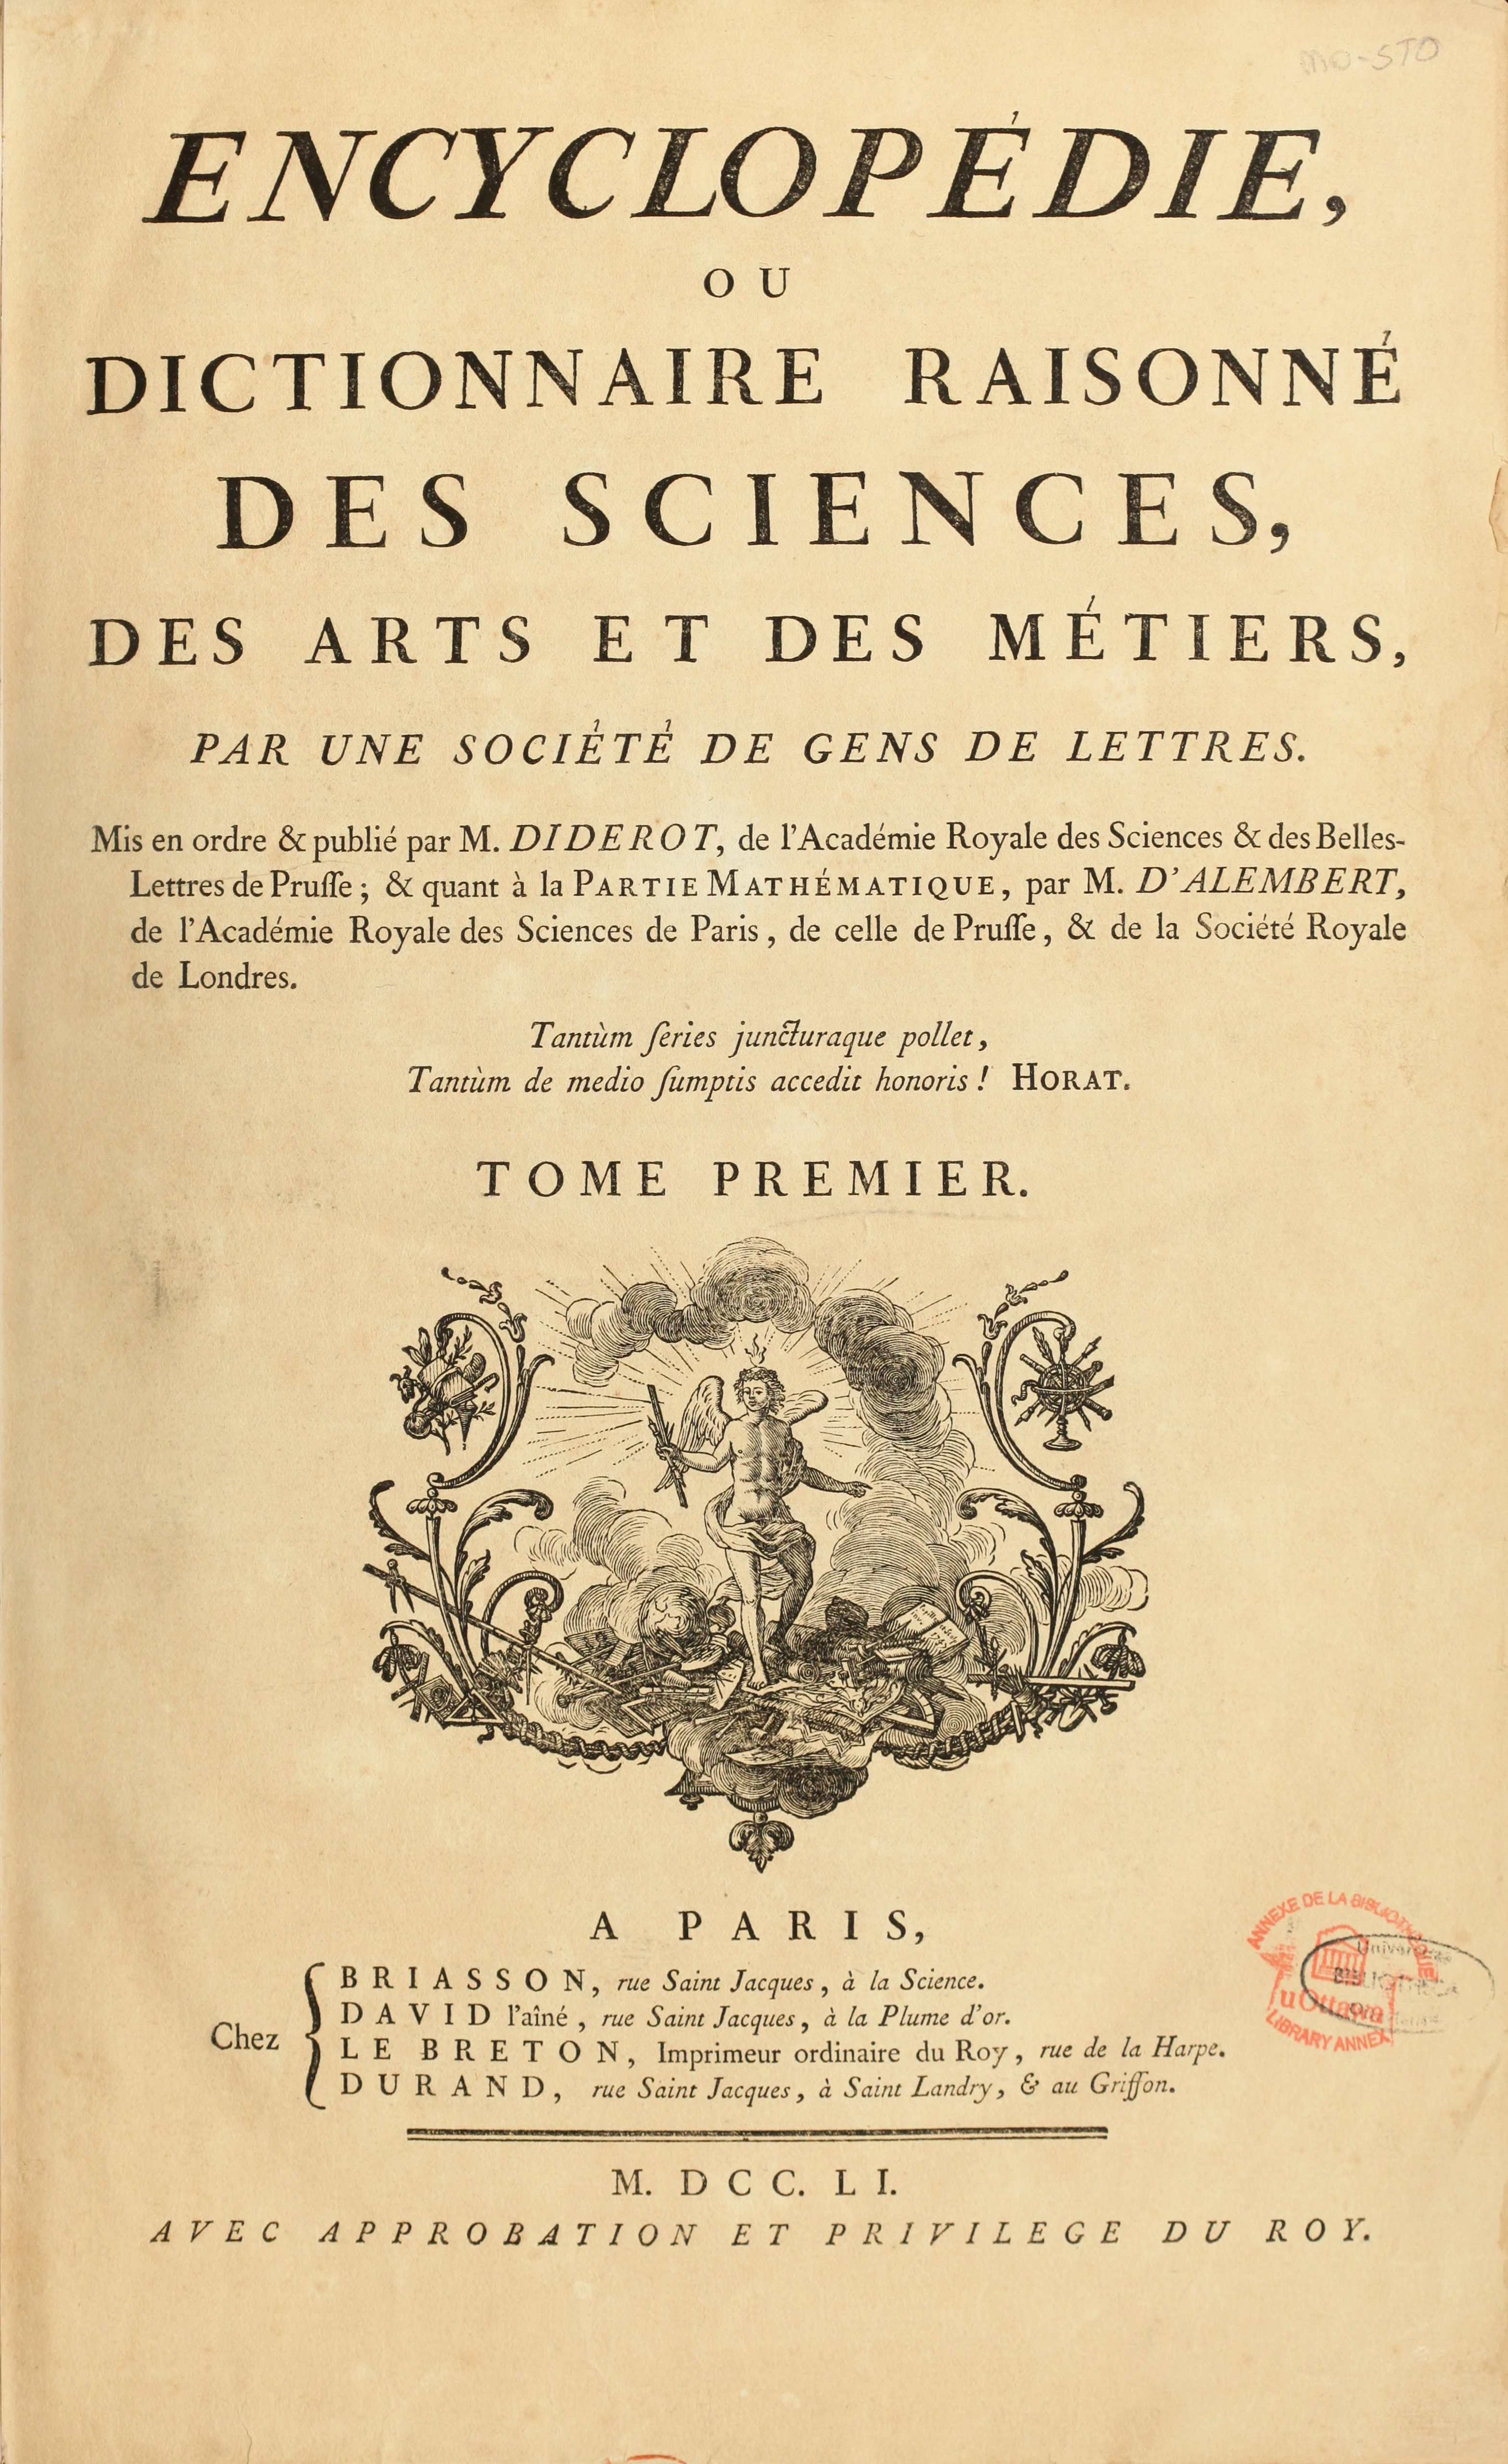
\includegraphics[height=80mm]{./images/Enciclopedia_portada.jpg}}
\vspace{10mm}
\subfigure[Estructura organizada del conocimiento humano. 1752]{\includegraphics[width=80mm, height=110mm]{./images/Conocimiento_humano.jpeg}}

\caption{Árbol de la ciencia de Llull y l'Encyclopédie de Diderot y d'Alembert}\label{fig:Enciclopedia}
\end{figure}

\section{Título del proyecto}

En la portada ---y otras páginas de presentación--- el nombre o título del
proyecto debe aparecer sin comillas, cursiva u otros formatos. Si se cita el
título de otra obra, o el nombre de un capítulo sí debe aparecer entre
comillas. Por cierto, las comillas que deben usarse en castellano son las
«latinas», dejando las ``inglesas'' para los raros casos en los que aparezca una
cita en el cuerpo otra~\cite{sousa}.


\section{Estructura del documento}

Pueden incluirse aquí una sección con algunos consejos para la lectura del
documento dependiendo de la motivación o conocimientos del lector.  También
puede ser útil incluir una lista con el nombre y finalidad de cada uno de los
capítulos restantes.

\begin{definitionlist}
\item[Capítulo \ref{chap:antecedentes}: \nameref{chap:antecedentes}] Explica herramientas
  y aspectos básicos de edición con \LaTeX.
\item[Capítulo \ref{chap:objetivos}: \nameref{chap:objetivos}] Finalidad y justificación
  (con todo detalle) del presente documento.
\end{definitionlist}


\section{Más texto para que ocupe varias páginas}

\blindtext
\blinditemize[4]
\blindmathpaper


% Local Variables:
%  coding: utf-8
%  mode: latex
%  mode: flyspell
%  ispell-local-dictionary: "castellano8"
% End:
